\documentclass[10pt,letterpaper]{article}
\usepackage[top=0.85in,left=2.0in,footskip=0.75in]{geometry}
\usepackage{amsmath,amssymb}
\usepackage{changepage}
\usepackage[utf8]{inputenc}
\usepackage{textcomp,marvosym}
\usepackage{cite}
\usepackage{nameref}
\usepackage[pdftex,
            pdfauthor={Peter Reintjes},
            pdftitle={Fitness Landscape Visualization},
            pdfsubject={MatPlotLib Visualization},
            pdfkeywords={Python Matplotlib},
            pdfproducer={Latex with hyperref},
            pdfcreator={pdflatex}]{hyperref}

\hypersetup{
    colorlinks=true,
    linkcolor=blue,
    filecolor=magenta,      
    urlcolor=cyan,
}
\usepackage[right]{lineno}
\usepackage{microtype}
\DisableLigatures[f]{encoding = *, family = * }
\usepackage[table]{xcolor}
\usepackage{array}
\usepackage{listings}
\newcolumntype{+}{!{\vrule width 2pt}}
\newlength\savedwidth
\newcommand\thickcline[1]{%
  \noalign{\global\savedwidth\arrayrulewidth\global\arrayrulewidth 2pt}%
  \cline{#1}%
  \noalign{\vskip\arrayrulewidth}%
  \noalign{\global\arrayrulewidth\savedwidth}%
}

% \thickhline command for thick horizontal lines that span the table
\newcommand\thickhline{\noalign{\global\savedwidth\arrayrulewidth\global\arrayrulewidth 2pt}%
\hline
\noalign{\global\arrayrulewidth\savedwidth}}

\usepackage{enumitem}
\setlist{nosep}
\raggedright
\setlength{\parindent}{0.5cm}
\textwidth 5.25in 
\textheight 8.75in

\usepackage[aboveskip=1pt,labelfont=bf,labelsep=period,justification=raggedright,singlelinecheck=off]{caption}
\renewcommand{\figurename}{Fig}

% Remove brackets from numbering in List of References
\makeatletter
\renewcommand{\@biblabel}[1]{\quad#1.}
\makeatother

% Leave date blank
\date{}
% Header and Footer with logo
\usepackage{lastpage,fancyhdr,graphicx,wrapfig}
\usepackage{epstopdf}
\pagestyle{myheadings}
\pagestyle{fancy}
\fancyhf{}
\setlength{\headheight}{27.023pt}
%\lhead{\includegraphics[width=2.0in]{PLOS-submission.eps}}
%\rfoot{\thepage/\pageref{lastpage}}
\renewcommand{\footrule}{\hrule height 2pt \vspace{2mm}}
\fancyheadoffset[L]{2.25in}
\fancyfootoffset[L]{2.25in}
% customize
\lfoot{\sf Innatrix Internal Document}

\begin{document}

\title{Fitness Landscape Animation Software}
\author{Peter Reintjes}
\date{\today}
\maketitle

\vspace*{0.2in}
\begin{flushleft}
\includegraphics[scale=0.5]{{fitness}.png}
\end{flushleft}

{\it Continuous Directed Evolution can be visualized by showing mutations as entities crawling across a fitness landscape until they come to a particular height on a fitness peak.  The two-dimensional surface is an imperfect representation of sequence space, which could be thought of as NxM dimensional space for the M possible substitutions for each of the N amino acids making up the protein sequence.  For a 1000 amino acid protein, this surface would be $1000 \times 1000^{21}$ points and would probably be quite spikey, as sequences(mutations) close to each other in this 2D representation would not necessarily have similar 'fitness'.  On the other hand, for directed evolution, the fitness is often a single quantity (say, protein-protein affinity) and is well represented by a height.  Thus the term fitness-peak to represent maxima in this space.  We use the Python matplotlib library\cite{matplotlib} program to create a series of static images, representing a particular population of mutations at one point in time.  These images are then assembled into a movie (GIF) image file to visualize the process of evolution.  This method was inspired by the animations created by Randy Olsen and Bjorn Ostman which can be found on the Wikipedia page for Fitness Landscape\cite{fitness}.}

\section*{Introduction}

The {\bf landscape.py} program is a Python program which generates a series of images representing snapshots of protein evolution.

\section*{Using MatPlotLib}

\begin{enumerate}[itemsep=1pt, topsep=2pt, partopsep=0pt]
\item Python/Matplotlib is free
\item Python/Matplotlib is portable between Windows and Linux systems
\item Skilled Python Programmers are becoming more numerous
\item Python was already in use for the EvoStat project
\item The MatLab/Octave alternative required an additional learning curve and those languages did not seem to suit other general purpose needs of the overall project.
\end{enumerate}
Although Octave, as an open-source alternative to MatLab is free and portable between systems, I decided to go with Python after initially prototyping in Octave.

\subsection*{Requirements}
The list of Python dependencies is large and so setting up the Python environment to have compatible versions of all required libraries has been a bit of a task.
\begin{lstlisting}
from __future__ import print_function
import numpy as np
import mpl_toolkits.mplot3d as a3
import pylab as pl
import scipy as sp
import matplotlib.pyplot as plt
import matplotlib.patches as mpatches
import matplotlib.colors as colors
import matplotlib
import random, glob, os, subprocess, sys
from shutil import copyfile
from mpl_toolkits.mplot3d import Axes3D
from matplotlib.colors import LightSource
\end{lstlisting}
\subsubsection*{ImageMagick}
Whenever ten additional static frames have been created, the program calls the ImageMagic\cite{imagemagick} {\tt convert} command:
\begin{lstlisting}
convert 0*.png -delay 12 -gravity Center -crop 500x280+20-20! out.gif
\end{lstlisting}
Which collects all of the properly cropped {\bf .png} files (in the /tmp/gifmovie directory) into an animated GIF with 12ms per frame.  This external command is called via the Python subprocess module, but could presumably be done using the PythonMagick bindings.  As this would also provide access to the other image enhancement features of ImageMagick this may be worth serious consideration.

\subsection*{Markers}
I chose the 'o' (circle), 'D' (diamond), and 's' (square) markers to represent the mutants, global maximum fitness peak, and landscape origin. But other markers could be chosen. There is an interesting outstanding problem with z-ordering the markers when drawn on top of a 3D surface.

\begin{wrapfigure}{L}{0.25\textwidth}
\centering
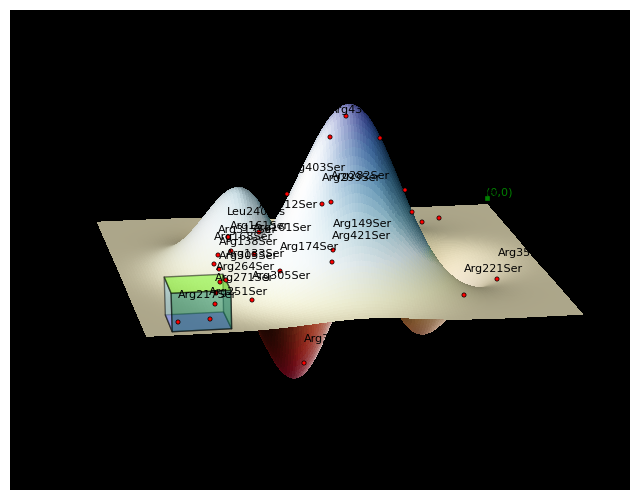
\includegraphics[width=0.23\textwidth,scale=0.2]{fitness.png}
\caption{\label{fig:reticules}A Single Snapshot}
\end{wrapfigure}

\section*{Next Steps}

I'm turning this project over to Dawn Trembath.

\begin{enumerate}[itemsep=1pt, topsep=2pt, partopsep=0pt]
\item Review/re-write code: can probably be halved.
\item Add command-line options to avoid frequent program edits
\item Consider cost/benefits of using PythonMagick bindings
\end{enumerate}

\bibliographystyle{unsrt}
\bibliography{landscape}{}

\pagebreak

\section{Appendix: landscape.py source code}
\newcommand*{\SrcPath}{..}
\lstinputlisting[language=Python]{\SrcPath/mlandscape.py}
\end{document}
